%%
%% Author: andre
%% 21/05/18
%%

% Preamble
\documentclass[11pt]{article}
\usepackage{basic}

\title{Descrição do sistema Nação Real}
\date{\today}

% Document
\begin{document}
    \maketitle
    \tableofcontents
    \listoffigures
    \newpage

    \section{Introdução}
    \label{s-intro}

    Esse sistema destina-se à melhor articulação intra e inter células. Buscamos criar um sistema de comunicação para
    que as ações estejam melhor coordenadas.

    \section[DER]{Diagrama Entidade-Relacionamento}
    \label{DER}

    \begin{figure}
        \centering
        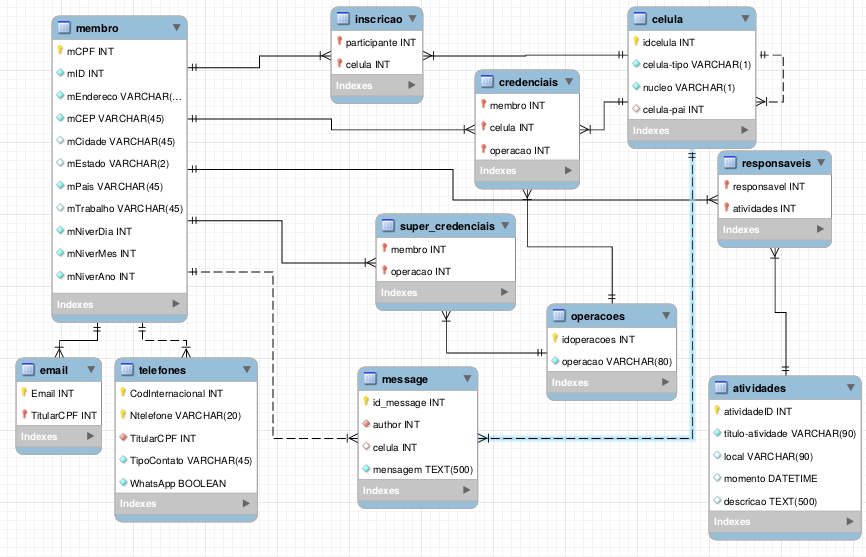
\includegraphics[width=0.85\textwidth]{bd.png}
        \caption{Diagrama que retrata as entidades}
        \label{fig:der}
    \end{figure}

    (Vide figura \ref{fig:der})

    \section[Dependências]{Descrição de dependências}

    Aqui encontra-se uma lista de dependências desse projeto:
    \begin{itemize}
        \item PostgreSQL \dir SGBD \footnote{sistema de gerenciamento de banco de dados}
        responsável pelo armazenamento de dados e transações referentes às operações de
        inserção, leitura, atualização e remoção
        \item psycopg2 \dir biblioteca Pyhton para comunicação com o SGBD
        \item Flask-RESTPlus \dir criação de rotas e requisições REST
        \item Axios \dir parte do front-end, recebem entrada em JSON e trazem os dados de
        forma nítida
        \item Vue \dir ferramenta de front-end, embelezamento
    \end{itemize}
    Abaixo encontram-se instruções de instalação. Tentarei incluir instruções de instalação
    para ambientes Unix/Linux. Caso acharem necessário ou mesmo conveniente, podem colocar
    instruções de instalação em Windows e macOS .

        \subsection{PostgreSQL}
        \subsection{Psycopg2}
        \subsection{Flask-RESTPlus}
        \subsection{Axios}
        \subsection{Vue}

    \section[Descrição]{Entidades e relacionamentos}

        \subsection{Membros}
            \begin{lstlisting}
                CREATE TABLE IF NOT EXISTS nacao_real.membro (
                    mID             SERIAL      NOT NULL,
                    mCPF            BIGINT      NOT NULL  UNIQUE,
                    mNome           VARCHAR(30) NOT NULL,
                    mSnome          VARCHAR(30) NOT NULL,
                    mEndereco       VARCHAR(90) NOT NULL,
                    mCodPostal      VARCHAR(9)  NOT NULL,
                    mCidade         VARCHAR(45) NOT NULL,
                    mEstado         VARCHAR(2)  NOT NULL,
                    mPais           VARCHAR(45) NOT NULL,
                    mESpecialidade  VARCHAR(45) NOT NULL,
                    mNasc           TIMESTAMP   NOT NULL,
                    mPassword       VARCHAR(90) NOT NULL
                    PRIMARY KEY (mID)
                );
            \end{lstlisting}

            Trata-se da entidade principal do BD. Abaixo estão seus atributos e informações
            relevantes:
            \begin{itemize}
                \item \cp \atr{mID} -- inteiro -- identificador serial de tuplas
                \item \atr{mCPF} -- inteiro grande -- escolhido para representar o CPF
                de uma pessoa. Ainda que o CPF possa ser melhor representado por uma string,
                acredito que a indexação seja mais otimizada se processsada com inteiros.
                A principal razão desse campo não ter sido escolhido como chave primária
                é o fato de que a chave primária ser utilizada nas requisições e procedimentos.
                Isso pode tornar-se uma fragilidade de segurança, se considerarmos que, dependendo
                do protocolo utilizado, essa informação pode ficar exposta
                \item \atr{mEndereco} -- string -- endereço do membro. Deve conter, pelo
                menos, o nome da rua, avenida ou o que for.
                \item \atr{mCodPostal} -- string -- representa o código postal de onde a pessoa
                mora. Pode incluir uma funcionalidade de identificação de endereço através do CEP
                \item \atr{mCidade} -- string -- representa a cidade de residência da pessoa
                \item \atr{mEstado} -- string -- representa o estado ou provícia de residência
                da pessoa
                \item \atr{mPais} -- string -- representa o país de residência da pessoa
                \item \atr{mESpecialidade} -- string -- campo importante, onde o usuário
                descreve sua área de formação. Muito útil para pesquisar quem lhe pode ser
                útil pra um determinado fim dentro da organização
                \item \atr{mNasc} -- data -- serve para verificar a idade dos membros.
                Possibilidades de agregar jovens lideranças, e agrupamento por idades
                \item \atr{mPassword} -- string -- devemos nos juntar e verificar condições de senha
                \item \criar O próprio usuário ou um administrador
                \item \ler Todos os usuários que estiverem numa mesma
                célula e os administradores.
                \item \atualizar Somente o próprio usuário
                \item \deletar O próprio usuário ou o administrador.
            \end{itemize}

        \subsection{Habilidades}

            Tabela representa o múltiplos valores que o campo habilidades e conhecimento podem ter

        \subsection{Células}
        \subsection{Mensagens}
        \subsection{Atividades}
        \subsection{Operações}

    \section[Equipe]{Membros da equipe}

    Nossa equipe é formada pelos seguintes membros
    \begin{itemize}
        \item André Luiz Abdalla Silveira
        \item Insira o nome de vocês no arquivo \LaTeX
    \end{itemize}

\end{document}
